\subsubsection{Kunnskapsutveksling}
EiT legger opp til at alle medlemmene som jobber med prosjektet skal få et faglig utbytte.
Både innenfor sine egne fagområder og resten av gruppens.
For å oppnå dette ønsket gruppen at det skulle være lett å dele den kunnskapen de enkelte medlemmene satt inne med med fra før.
Så tidlig som 2. landsbydag utarbeidet gruppen en samarbeidskontrakt.
Målet var å oppnå en felles oppfatning innad i gruppen om hvordan gruppearbeidet skulle utføres.
I tillegg skulle den bestemme hvilke krav gruppens medlemmer kunne stille til hverandre.
Hovedemnene var leveranse, læring og trivsel.
Samarbeidsavtalen ligger i vedlegg \ref{Ved:samarbeidsavtale}.
Viktigheten av god kommunikasjon innad i gruppen ble gjenspeilet i flere punkter i kontrakten. 

Et viktig poeng med EiT er tverrfaglig samarbeid. Dette målet ble reflektert i punkt 8 i samarbeidskontrakten: \textit{Gruppen skal drive kunnskapsutveksling gjennom diskusjon og drøfting av faglig innhold, samt utfordre hverandre til å gå utenfor den faglige komfortsonen.} Blant annet ville det være viktig å utnytte Ingelin sine kunnskaper om generell kjemi for at resten av gruppen skulle komme raskt igang med arbeidet.
Flere av gruppemedlemmene har vært takknemlig for hvor enkelt det har vært å spørre om andres kompetanse under prosjektarbeidet.
Karsten som har jobbet mye med de biologirettede delene av prosjektrapporten har gitt uttrykk for at Ingelin sine forhåndskunnskaper var til stor hjelp, og at Ingelin var villig til å avbryte eget arbeid for å hjelpe til.
Det er også av interesse å høre hva de ulike gruppemedlemmene har av faglige lidenskaper for å kunne skape et godt sosialt og løsningsorientert miljø i gruppen. \\

Kommunikasjon er ikke bare muntlig kunnskapsutveksling, ei heller formelt nødvendigvis.
Et eksempel på hvordan dette har foregått er de tekniske løsningene rundt dokumentdeling og ferdigstilling av prosjekt- og prosessrapporten.
For å legge til rette for individuelt arbeid valgte gruppen å bruke en programvare som heter Git.
Dette programmet sørger for versjonskontroll og at dokumentene ble delte samt oppdaterte.
Programvaren tok litt tid å sette opp, men etter dette har medlemmene kunnet skrive selvstendig samtidig som det ikke var behov for å bekymre seg for at noen andres arbeid ble slettet i prosessen.
Ferdigstillingen av rapportene har blitt gjort i \LaTeX.
Begge disse tekniske løsningene har hatt noen implementeringsutfordringer som Jonas og Martin har jobbet med underveis.
Det har krevd at de begge bidro med å dele sin forhåndskunnskap og samarbeide om å finne ny informasjon som kunne belyse problemer som oppstod underveis.


Siden samarbeidsavtalen var noe som ble utviklet tidlig, og før prosjektarbeidet hadde kommet skikkelig i gang, er det vanskelig å se om dette punktet har ført til noen vesentlig utvikling i gruppen.
Likevel viser dette seg å være en av flere årsaker til åpen kommunikasjon i gruppen. \\

\subsubsection{Kommunikasjonsdynamikk}

Trenden med at medlemmene i gruppen hadde ulik mengde initiativ i diskusjoner var grunnlag for regel \#11.: \textit{Alle i gruppen skal vise hverandre respekt. Dette gjennom å lytte, bidra med egne meninger, gi konstruktiv kritikk og bygge videre på andres id\'{e}er.} 
Gruppen består av medlemmer som opprinnelig hadde veldig ulike \textit{tilnærminger} til åpne diskusjoner og samtaler.
For eksempel sier både Karsten og Jonas at de er klar over at de tar mye initiativ og \textit{tar stor plass} i diskusjoner.
Derimot forholder Simen og Ingelin seg forholdsvis stille, og tar gjerne ikke ordet like ofte.
Anna og Martin plasserer seg omtrent midt mellom de to andre \textit{grupperingene}.
Dette mønsteret i kommunikasjonen er noe gruppen var klar over ganske tidlig, og har jobbet med i løpet av prosjektperioden.
Som Jonas skriver i refleksjonen om hva han lærte om gruppen i løpet av 14. januar:
"Vi har veldig ulike bakgrunner, både sosialt og faglig. Likevel virker alle åpne. Det er flere av oss som liker å ta ordet. Det er en bra start, men vi må være obs. på at alle får sagt det de ønsker."
En aksjon for å oppnå punkt \#11 var å la ordet gå på rundgang rundt bordet når viktige avgjørelser skulle tas. Da fikk alle medlemmene muligheten til å legge frem sitt synspunkt. På denne måten ble også medlemmene \textit{tvunget} til å ha en mening om alt som ble diskutert.

For å kontrollere den naturlige dynamikken i gruppen, ble punkt \#10: \textit{Gruppen skal ha rullerende møteleder og sekretær for hver landsbydag. Møteleder har hovedansvar for å overse arbeidsplan og trivsel samt å være ordstyrer.}, innført både som aksjon for å oppnå punkt \#11 og for å bli mer tidseffektive. En ordstyrer vil kunne fordele taletid mellom alle medlemmene i gruppen, og også oppmuntre medlemmer som har vært stille lenge til å komme med innspill. Dette punktet i kontrakten ble overholdt gjennom hele EiT-perioden. Ved å innføre ordningen har kommunikasjonen trolig vært mer åpen og flytende enn uten.

\subsubsection{Semantisk støy}

Øvelsen SITRA gikk ut på at gruppemedlemmene leste to fiktive refleksjoner av en og samme situasjon.
Medlemmene skulle først individuelt kategorisere setningene som situasjon, refleksjon, aksjon eller teori.
Deretter skulle tolkningene sammenlignes og diskuteres felles i gruppen.
Denne øvelsen trente gruppemedlemmene i kommunikasjon, og da spesielt i problemene som oppstår ved semantisk støy.
Semantisk støy handler om hvordan ord og uttrykk blir tolket.
Til å begynne med var det store ulikheter i oppfatningene av hva som hørte til i hver kategori.
Det krevdes derfor diskusjon og presisjon fra hvert medlem om hvor skillet mellom de ulike kategoriene skulle være.
Øvelsen viste hvor viktig det er å forklare andre medlemmer hva som menes med ulike begreper. 
Dette faktum er også tydeliggjort i \textit{Roger Schwarz} sine \textit{Grunnregler for effektive grupper}\cite{schwarz}. 
Han poengterer viktigheten av å sjekke antagelser og slutninger som trekkes fra det andre presenterer til deg. 
Det trekkes flere slutninger daglig, ofte automatisk og uten å være gjennomtenkt. 
Uten å være klar over det, kan slutningene oppfattes som fakta.
Dermed kan misforståelser oppstå, ved at deler av budskapet er blitt stengt ute eller mistolket. Intensjonene til den andre kan dermed tolkes feilaktig i forhold til personens egentlige budskap.
Hvis det er tvil om intensjoner og budskap, må medlemmene ikke nøle med å spørre om alt er forstått korrekt. Ved hjelp av SITRA øvelsen ble gruppen for første gang introdusert for viktigheten av å presisere hva som legges i begreper. 

Under grupperefleksjonen landsbydag syv, diskuterte Anna og Karsten oppgavene til referentsrollen. Begge tolket hverandres synspunkter for fort uten å ha forstått den andres egentlige budskap. Det resulterte i at de trodde den andre hadde motsatte intensjoner, mens de faktisk hadde veldig like synspunkt om hva referenten hadde som oppgave. 

\begin{center}
	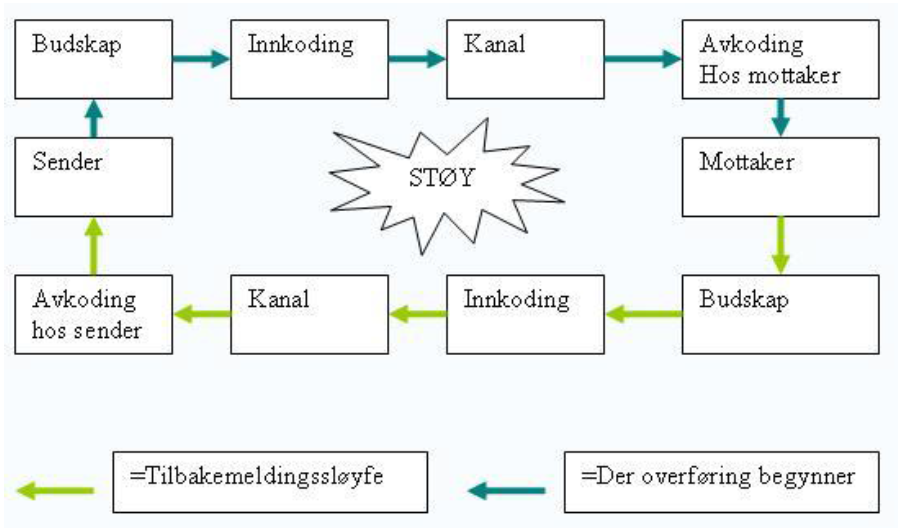
\includegraphics[width=0.5\textwidth]{Kommunikasjon.PNG}
\end{center}


Hvis sender og mottaker operer med ulike referanserammer så kan budskapet bli tolket på en annen måte enn det var tiltenkt, eller det kan bli fullstendig uforståelig \cite{prosjekteringsledelse}.
Formålet med SITRA-øvelsen var å bevisstgjøre gruppa på disse referanserammene.

Et mer gjennomgående og ikke-iscenesatt eksempel på dette er at Anna og Karsten har andre morsmål.
Dette har latt gruppen oppleve, ved flere anledninger, hva semantisk støy betyr.
 -grunnregler for effektive grupper: spesielt formulere seg korekkt og ikke bli mistolket : Anna og Karsten
 
\subsubsection{Sosiale inntrykk}

Analysere sosiogram + sosiale inntrykk Anna

Andre kommunikasjonstrender som har blitt observert i gruppen er en økt grad av frie samtaler, småprat og humor. Spesielt Martin og Karsten har hatt lett for å skape digresjoner, slik at resten av gruppen har måttet be dem om å beholde fokus. 
Kommunikasjonsmønsteret i gruppen har under hele prosessen endret seg.
Noen ganger gradvis og sakte, andre ganger raskere. 




























